\documentclass[review]{elsarticle}

\usepackage{lineno,hyperref}
\modulolinenumbers[5]

\usepackage{amssymb}
\usepackage{graphicx}
%\usepackage{autonum}
\usepackage{amsmath}
\usepackage{caption}
\usepackage{subcaption}
\captionsetup[table]{skip=10pt}

%\usepackage{url}
% ********************************** Tikz & PGF plots *************************
\usepackage{pgfplots}

\usepackage{tikz}
\usetikzlibrary{decorations.pathmorphing} % noisy shapes
\usetikzlibrary{fit}                    % fitting shapes to coordinates
\usetikzlibrary{backgrounds}    % drawing the background after the foreground
\usetikzlibrary{shapes, arrows}


% The input, state transition, and measurement matrices
% are represented by gray squares.
% They have a smaller minimal size for aesthetic reasons.
\tikzstyle{matrx}=[rectangle, thick, minimum size=1.0cm, draw=gray!80,
                   fill=gray!20] 

% Everything is drawn on underlying gray rectangles with
% rounded corners.
\tikzstyle{background}=[rectangle, draw=gray!40, fill=gray!10, inner
                        sep=0.1cm, rounded corners=1mm]
% *****************************************************************************

%\usepackage{autonum}
\usepackage{subcaption} % For subfigures
\captionsetup{compatibility=false}

\newtheorem{assumption}{Assumption}
\journal{Journal of \LaTeX\ Templates}

%%%%%%%%%%%%%%%%%%%%%%%
%% Elsevier bibliography styles
%%%%%%%%%%%%%%%%%%%%%%%
%% To change the style, put a % in front of the second line of the current style and
%% remove the % from the second line of the style you would like to use.
%%%%%%%%%%%%%%%%%%%%%%%

%% Numbered
%\bibliographystyle{model1-num-names}

%% Numbered without titles
%\bibliographystyle{model1a-num-names}

%% Harvard
%\bibliographystyle{model2-names.bst}\biboptions{authoryear}

%% Vancouver numbered
%\usepackage{numcompress}\bibliographystyle{model3-num-names}

%% Vancouver name/year
%\usepackage{numcompress}\bibliographystyle{model4-names}\biboptions{authoryear}

%% APA style
%\bibliographystyle{model5-names}\biboptions{authoryear}

%% AMA style
%\usepackage{numcompress}\bibliographystyle{model6-num-names}

%% `Elsevier LaTeX' style
\bibliographystyle{elsarticle-num}
%%%%%%%%%%%%%%%%%%%%%%%

\begin{document}

\begin{frontmatter}

\title{Generalised Classification Restricted Boltzmann Machines}
%\tnotetext[mytitlenote]{We thank Dr Srikanth Cherla for his public code on discriminative RBMs.}


\author[mymainaddress]{Son N. Tran\corref{mycorrespondingauthor}\fnref{myfootnote}}
\cortext[mycorrespondingauthor]{Corresponding author}
\ead{son.tran@csiro.au}
\fntext[myfootnote]{Level 5 UQ Health Sciences Building,  Royal Brisbane and Women's Hospital,
  Herston, Queensland 4029 Australia}
\address[mymainaddress]{The Australian E-Health Research Centre, CSIRO}

%% Group authors per affiliation:
\author[mysecondaryaddress]{Chadi Hajj\fnref{mysecondaryfootnote}}
\author[mysecondaryaddress]{Artur Garcez\fnref{mysecondaryfootnote}}
\author[mysecondaryaddress]{Tillman Weyde\fnref{mysecondaryfootnote}}
\fntext[mysecondaryfootnote]{College Building, Northampton Square, London, EC1V 0HB, United Kingdom}
\address[mysecondaryaddress]{Department of Computer Science, City University of London}

%% or include affiliations in footnotes:

\begin{abstract}
Here goes the abstract
\end{abstract}

\begin{keyword}
Restricted Boltzmann machines, Classification
\MSC[2010] 00-01\sep  99-00
\end{keyword}

\end{frontmatter}

\linenumbers
\section{Introduction}
\label{sec:introduction}
The restricted Boltzmann machine (RBM) is a generative latent-variable
model which models the joint distribution of a set of input variables.
It has gained popularity over the past decade in many applications,
especially for pretraining deep neural network classifiers
\cite{Hinton_2006,Mohamed2012}.  One of its applications is as a
standalone classifier, referred to as the Discriminative Restricted
Boltzmann Machine (DRBM)\cite{Larochelle2008}.  As the name might
suggest, the DRBM is a classifier obtained by carrying out
discriminative learning in the RBM and it directly models the
conditional distribution one is interested in for prediction. This
bypasses one of the key problems faced in learning the parameters of
the RBM generatively, which is the computation of the intractable
\textit{partition function}.  In the DRBM this partition function is
cancelled out in the expression for the conditional distribution thus
simplifying the learning process.

It is often the case that a new type of activation function results in
an improvement in the performance of an existing model or in a new
insight into the behaviour of the model itself.  In the least, it
offers researchers with the choice of a new modelling alternative. In
fact, different type of units such as bipolar Bernoulli
\cite{Freund1992}, Gaussian \cite{Welling2004}, Binomial
\cite{Teh2001} and rectified linear \cite{Nair2010} have been
studied. However, we observe that while effort has gone into enhancing
the performance of a few other connectionist models by changing the
nature of their hidden units, this has not been attempted with the
DRBM.  So in this paper, we first describe a novel theoretical result
that makes it possible to generalise the model's cost function.  The
result is then used to derive two new cost functions corresponding to
DRBMs containing hidden units with the Binomial and $\{-1,
+1\}$-Bernoulli distributions respectively.  These two variants are
evaluated and compared with the original DRBM on the benchmark MNIST
and USPS digit classification datasets, and the 20 Newsgroups document
classification dataset.  We find that each of the three compared
models outperforms the remaining two in one of the three datasets,
thus indicating that the proposed theoretical generalisation of the
DRBM may be valuable in practice.
    
In the next Section, we explain the generalisation of the
discriminative function in RBMs. It is followed by Section
\ref{subsec:drbm_extensions} that shows how to implement this
idea. Experimental results are discussed in Section
\ref{sec:experiments} and Section \ref{sec:conclusions} presents a
summary, together with potential extensions of this work

\section{Related Work}
\label{sec:relate}


\section{Generalised Classification Restricted Boltzmann Machines}
\subsection{Model}
\begin{figure}[ht]
  \centering
  \begin{subfigure}[b]{0.45\textwidth}
    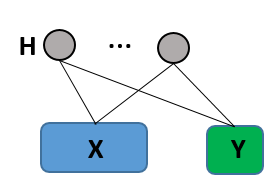
\includegraphics[scale=1]{crbm.png}
    \subcaption{Classification RBMs}
  \end{subfigure}
  \begin{subfigure}[b]{0.45\textwidth}
    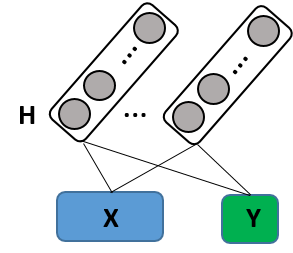
\includegraphics[scale=1]{gcrbm.png}
    \subcaption{Generalised classification RBMs}
  \end{subfigure}
\end{figure}

The Restricted Boltmzann Machine (RBM) \cite{Smolensky1986} is an
undirected bipartite graphical model. In the case for classification,
it contains a set of visible units $\mathbf{v}=\{\mathbf{x} \in
\mathbb{R}^{n_x},\mathbf{y} \in \mathbb{R}^{n_y}\}$, where
$\mathbf{x}$ is the input vector, and $\mathbf{y}$ is the one-hot
encoding of the class-label; and a set of hidden units $\mathbf{h} \in
\mathbb{R}^{n_h}$.  The two layers are fully inter-connected but there
exist no connections between any two hidden units, or any two visible
units.  Additionally, the units of each layer are connected to a bias
unit whose value is always 1.  The edge between the $i^{th}$ input
$x_i$ and the $j^{th}$ hidden unit $h_j$ is associated with a weight
$w_{ij}$. All these weights are together represented as a weight
matrix $W \in \mathbb{R}^{n_x \times n_h}$. Similarly, $U \in
\mathbb{R}^{n_y\times n_h}$ is the weight matrix between labels
$\mathbf{y}$ and the hidden layer $\mathbf{h}$.  The weights of
connections between input and label units and the bias unit are
contained in bias vectors $\mathbf{a} \in \mathbb{R}^{n_x}$,
$\mathbf{b} \in \mathbb{R}^{n_y}$ respectively.  Likewise, for the
hidden units there is a hidden bias vector $\mathbf{c} \in
\mathbb{R}^{n_h}$.  The RBM is characterized by an energy function: $
E(\mathbf{x},\mathbf{y}, \mathbf{h}) = -\mathbf{a}^{\top}\mathbf{x}
-\mathbf{b}^{\top}\mathbf{y} - \mathbf{c}^{\top}\mathbf{h} -
\mathbf{x}^{\top}W\mathbf{h} - \mathbf{y}^\top U\mathbf{h}$ to
represent the joint probability of every possible pair of visible and
hidden vectors as: $ P(\mathbf{x},\mathbf{y}, \mathbf{h}) =
\frac{1}{Z} \mathrm{e}^{-E(\mathbf{x},\mathbf{y}, \mathbf{h})}$ where
$Z$ is the partition function, $ Z = \sum_{\mathbf{x},\mathbf{y},
  \mathbf{h}} \mathrm{e}^{-E(\mathbf{x},\mathbf{y}, \mathbf{h})}$.


....  Normally, RBMs can have binary units or Gaussian units
\cite{}. However, the latter is difficult to use for classification
since different from the binary hidden units in RBMs
with Gaussian hidden units $p(y|\mathbf{x})$ is intractable. We can ... in
\cite{} to extend binary hidden units to represent binomial
distribution.

...

An RBM with binomial hidden units can be constructed by replicating
each hidden unit N times \cite{}. Let us denote $h_j \in \{0,1,
...,N\}$ as a binomial hidden unit and each $h_j$ is represented by a
group of binary hidden unit $h_j^{(1)}$, $h_j^{(2)}$, ...,
$h_j^{(N)}$. The probability of activating a unit in this group is
$p_j$ where:
\begin{equation}
 p_j  =  \sigma(\mathbf{x}^\top W + b_j)
\end{equation}
 
Because the weights are shared between N replicas of hidden unit $j$
the probability of $n$ units are activated is:

\begin{equation}
  p(h_j=n|\mathbf{x}) = \begin{pmatrix}
  N \\
  n  
 \end{pmatrix} p_j^n(1-p_j)^{(N-n)} = Bi(h_j=n,N,p_j)
\end{equation}

So, one can say the group of N shared-weight hidden units represent
the binomial distribution given the state of the other layer.


Let us consider the case of discriminative learning where the label is
encoded as one hot vector $\mathbf{y}$, as in Figure \ref{}. The
energy function will look like:
\begin{equation}
\begin{aligned}
E(\mathbf{x},y,\mathbf{h}) &= -\sum_{ijk}x_iw_{ij}h^{(k)}_j -\sum_{jk}u_{yj}h^{(k)}_j - \sum_i x_i a_i - b_y - \sum_{jk}c_jh^{(k)}_j\\ 
 &= -\sum_{j}\sum_k h^{(k)}_j (\sum_i x_iw_{ij} - u_{yj} - c_j) - \sum_i x_i a_i - b_y
\end{aligned}
\end{equation}

For classification, learning is carried out by maximising a hybrid log-likelihood which combine the generative and discriminative functions:
\begin{equation}
\mathcal{L} = \mathcal{L}_{discriminative} + \alpha\times \mathcal{L}_{generative}
\end{equation}
\subsection{Generative Function}
\begin{equation}
 \mathcal{L}_{generative} = \frac{1}{N}\sum_n^N \log p(\vt{x}^{(n)},y^{(n)})
\end{equation}

\subsection{Discriminative Function}
In this paper, we are interested in the conditional function which is important for classification:

 \begin{equation}
   P(y|\mathbf{x}) = \frac{\sum_{\mathbf{h}} \exp\left(-E\left(\mathbf{x},
     \mathbf{y}, \mathbf{h}\right)\right)}{\sum_{\mathbf{y}^{*}}
     \sum_{\mathbf{h}} \exp\left(-E\left(\mathbf{x}, \mathbf{y}^{*},
     \mathbf{h}\right)\right)} 
   \label{eq:p_y_given_x}
 \end{equation}


The denominator sums over all class-labels $\mathbf{y}^*$ to make
$P(\mathbf{y} |\mathbf{x})$ a probability distribution.  In the
original RBM, $\mathbf{x}$ and $\mathbf{y}$ together make up the
visible layer.  The model is learned discriminatively by maximizing
the log-likelihood function based on the expression of the conditional
distribution above. Normally, such RBMs have binary states $\{0,1\}$
for the hidden units. We will show how to extend the conditional
distribution with different type of hidden units.

If an RBM whose hidden units have $K$ states $\{s_k|k=1:K, K \in \mathbb{Z}\}$ then its
conditional distribution in \eqref{eq:p_y_given_x} can be computed
analytically. We are interested in the conditional distribution
\begin{equation}
\label{eq:cond}
p(y|\mathbf{x}) = \frac{p(\mathbf{x},y)}{\sum_{y^*} p(\mathbf{x},y^*)}
\end{equation}

where 
\begin{equation}
\label{eq:cond1}
  p(\mathbf{x},y) = \frac{1}{Z}\sum_\mathbf{h}\exp(-E(\mathbf{x},y,\mathbf{h})
\end{equation}
Apply \eqref{eq:cond1} to \eqref{eq:cond} the partitional function $Z$
will be cancelled out such that:

\begin{equation}
\label{eq:cond2}
p(y|\mathbf{x}) = \frac{\sum_\mathbf{h}\exp(-E(\mathbf{x},y,\mathbf{h}))}{\sum_{y^*}\sum_\mathbf{h}\exp(-E(\mathbf{x},y^*,\mathbf{h}))}
\end{equation}

In order to compute the conditional function in \eqref{eq:cond2} we
need to find $\sum_\mathbf{h}\exp(-E(\mathbf{x},y,\mathbf{h}))$.

Here,

\begin{equation}
  \sum_\mathbf{h}\exp(-E(\mathbf{x},y,\mathbf{h})) = \exp(\sum_{h_1=0}^N ... \sum_{h_J=0}^N \large{(}\sum_{j}\sum_k h^{(k)}_j (\sum_i x_iw_{ij} + u_{yj} + c_j) + \sum_i x_i a_i + b_y \large{)})
\end{equation}

Let us consider the term:
\begin{equation}
  \sum_\mathbf{h}\exp(-E(\mathbf{x},y,\mathbf{h})) = \exp(\sum_{h_1=0}^N ... \sum_{h_J=0}^N \large{(}\sum_{j}\sum_k h^{(k)}_j (\sum_i x_iw_{ij} + u_{yj} + c_j))
\end{equation}

Note that if $h_j = n$ then there will be $n$ units in the group $h_j^{(1)}, ..,h_j^{(N)}$ activated and therefore 
\begin{equation}
\sum_k h^{(k)}_j (\sum_i x_iw_{ij} + u_{yj} + c_j) = n\alpha_j 
\end{equation}

 where $\alpha_j = (\sum_i x_iw_{ij} + u_{yj} + c_j)$

\begin{equation}
  \begin{aligned}
  \sum_\mathbf{h}\exp(-E(\mathbf{x},y,\mathbf{h})) &= \exp(\sum_{h_1=0}^N\sum_{h_2=0}^N ... \sum_{h_J=0}^N \sum_{j} h_j \alpha_j)\\
                                                   &= \prod_{h_1=0}^N\prod_{h_2=0}^N ... \prod_{h_J=0}^N \prod_{j}\exp( h_j \alpha_j))\\
                                                   & = \prod_j\sum_{h_j=0}^N \exp(h_j \alpha_j)
  \end{aligned}
\end{equation}

Now we denote $s_k$ as a state of the hidden unit such that $s_0 = 0$, $s_1 = 1$, ... the product $\prod_j\sum_{h_j=0}^N \exp(h_j \alpha_j)$ can replaced by $\prod_j\sum_{k=0}^N \exp(s_k \alpha_j)$.

where $s_k$ is each of the $k$ states that can be assumed by each
hidden unit $j$ of the model. The last step of (\ref{eq:transform})
results from re-arranging the terms after expanding the summation and
product over $\mathbf{h}$ and $j$ in the previous step
respectively. The summation $\sum_\mathbf{h}$ over all the possible
hidden layer vectors $\mathbf{h}$ can be replaced by the summation
$\sum_k$ over the states of the units in the layer.  The number and
values of these states depend on the nature of the distribution in
question.  The result
in (\ref{eq:transform}) can be applied to (\ref{eq:free_energy}) and,
in turn, to (\ref{eq:p_y_given_x}) to get the following general
expression of the conditional probability $P(y|\mathbf{x})$:

\begin{equation*}
\begin{aligned}
P(y|\mathbf{x}) &= \frac{\exp\left(b_y\right) \prod_j \sum_k \exp\left(s_k
                \alpha_j\right)}{\sum_{y^{*}} \exp\left(b_{y^{*}}\right) 
                \prod_j \sum_k \exp\left(s_k \alpha^*_j\right)} 
\end{aligned}
\end{equation*}


%Indeed, let us consider the term containing the summation over $\mathbf{h}$ in (\ref{eq:p_y_given_x}):
%\begin{equation}
%\begin{aligned}
% \sum_{\mathbf{h}} \exp\left(-E\left(\mathbf{x}, \mathbf{y},
% \mathbf{h}\right)\right) &= \sum_{\mathbf{h}}
% \exp\left(\sum_{i,j} x_i w_{ij} y_j + \sum_j u_{yj}h_j + \sum_i a_i  x_i + b_y + \sum_j c_j h_j\right) \\ &= \exp\left(\sum_i a_i x_i +
% b_y\right) \sum_{\mathbf{h}} \exp\left(\sum_j h_j \sum_i x_i w_{ij} +
% u_{yj} + c_j\right)
%\label{eq:free_energy}
%\end{aligned}
%\end{equation}
%Now consider only the second term of the product in
%(\ref{eq:free_energy}).  We simplify it by re-writing $\sum_i x_i w_{ij} + u_{yj} + c_j$ as $\alpha_j$.  Thus, we have:
%\begin{equation}
%\begin{aligned}
%\sum_{\mathbf{h}} \exp\left(\sum_j h_j \sum_i x_i w_{ij} + u_{yj} + c_j\right) &= \prod_j \sum_k \ex%p\left(s_k \alpha_j\right)
%\label{eq:transform}
%\end{aligned}
%\end{equation}
%where $s_k$ is each of the $k$ states that can be assumed by each
%hidden unit $j$ of the model. The last step of (\ref{eq:transform})
%results from re-arranging the terms after expanding the summation and
%product over $\mathbf{h}$ and $j$ in the previous step
%respectively. The summation $\sum_\mathbf{h}$ over all the possible
%hidden layer vectors $\mathbf{h}$ can be replaced by the summation
%$\sum_k$ over the states of the units in the layer.  The number and
%values of these states depend on the nature of the distribution in
%question.  The result
%in (\ref{eq:transform}) can be applied to (\ref{eq:free_energy}) and,
%in turn, to (\ref{eq:p_y_given_x}) to get the following general
%expression of the conditional probability $P(y|\mathbf{x})$:
%\begin{equation*}
%\begin{aligned}
%P(y|\mathbf{x}) &= \frac{\exp\left(b_y\right) \prod_j \sum_k \exp\left(s_k
%                \alpha_j\right)}{\sum_{y^{*}} \exp\left(b_{y^{*}}\right) 
%                \prod_j \sum_k \exp\left(s_k \alpha^*_j\right)} 
%\end{aligned}
%\end{equation*}
%Proposition \ref{prop} generalises the conditional probability of the
%DRBM first introduced in \cite{Larochelle2008}.  The term inside the
%summation over $k$ can be viewed as a product between $\alpha_j$
%corresponding to each hidden unit $j$ and each possible state $s_k$ of
%this hidden unit.  Knowing this makes it possible to extend the
%original DRBM to be governed by other types of distributions in the
%hidden layer, as what will be discussed in the next section.

\section{Model Instances}
\subsection{DRBM}
\label{subsubsec:logsig_act}
The $\{0, 1\}$-Bernoulli DRBM corresponds to the model originally
introduced in \cite{Larochelle2008}.  In this case, each hidden unit
$h_j$ can either be a $0$ or a $1$, i.e.  $s_k = \{0, 1\}$.  This
reduces $P(y|\mathbf{x})$ in (\ref{eq:drbm_generalisation}) to

 \begin{equation}
       % \begin{aligned}
                P_{\textrm{ber}}\left(y|\mathbf{x}\right) 
                =  \frac{\exp\left(b_y\right) \prod_j \left(1 +
                    \exp\left(\alpha_j\right)\right)} {\sum_{y^{*}}
                    \exp\left(b_{y^{*}}\right) \prod_j \left(1 +
                    \exp\left(\alpha^*_j\right)\right)} 
                % \end{aligned}
 \end{equation}

 which is identical to the result obtained in \cite{Larochelle2008}.
\subsection{Bipolar DRBM:}
\label{subsubsec:tanh_act}
%\vskip -.3cm
A straightforward adaptation to the DRBM involves replacing its hidden
layer states by $\{-1, +1\}$ as previously done in \cite{Freund1992}
in the case of the RBM.  This is straightforward because in both cases
the hidden states of the models are governed by the Bernoulli
distribution, however, in the latter case each hidden unit $h_j$ can
either be a $-1$ or a $+1$, i.e. $s_k = \{-1, +1\}$.  Applying this
property to (\ref{eq:drbm_generalisation}) results in the following
expression for $P(y|\mathbf{x})$:

\begin{equation}
 P_{\textrm{bip}}\left(y|\mathbf{x}\right) =
 \frac{\exp\left(b_y\right) \prod_j \left(\exp\left(-\alpha_j\right) +
   \exp\left(\alpha_j\right)\right)} {\sum_{y^{*}}
   \exp\left(b_{y^{*}}\right) \prod_j
   \left(\exp\left(-\alpha^*_j\right) +
   \exp\left(\alpha^*_j\right)\right)}
\end{equation}

\subsection{Binomial DRBM:}
\label{subsubsec:bin_act}
%\vskip -.5cm
It was demonstrated in \cite{Teh2001} how groups of $N$ (where $N$ is
a positive integer greater than $1$) stochastic units of the standard
RBM can be combined in order to approximate discrete-valued functions
in its visible layer and hidden layers to increase its
representational power.  This is done by replicating each unit of one
layer $N$ times and keeping the weights of all connections to each of
these units from a given unit in the other layer identical.  The key
advantage for adopting this approach was that the learning algorithm
remained unchanged.  The number of these ``replicas'' of the same unit
whose values are simultaneously $1$ determines the effective integer
value (in the range $[0, N]$) of the composite unit, thus allowing it
to assume multiple values.  The resulting model was referred to there
as the Rate-Coded RBM (RBMrate).
            
The intuition behind this idea can be extended to the DRBM by allowing
the states $s_k$ of each hidden unit to assume integer values in the
range $[0, N]$.  The summation in (\ref{eq:drbm_generalisation}) would
then be $S_N = \sum_{s_k=0}^N \exp\left(s_k \alpha_j\right)$, which
simplifies as below:

\begin{equation}
        %\begin{aligned}
S_N = \sum_{s_k=0}^N \exp\left(s_k \alpha_j\right) = \frac{1 - \exp\left(\left(N+1\right) \alpha_j\right)}{1 -
 \exp\left(\alpha_j\right)} 
           % \end{aligned}
\end{equation}

 in (\ref{eq:drbm_generalisation}) to give

 \begin{equation}
        %\begin{aligned}
                P_{\textrm{bin}}\left(y|\mathbf{x}\right) 
                = \frac{\exp\left(b_y\right) \prod_j
                    \frac{1-\exp\left(\left(N+1\right)
                    \alpha_j\right)}{1-\exp\left(\alpha_j\right)}} 
                    {\sum_{y^{*}} \exp\left(b_{y^{*}}\right) \prod_j
                    \frac{1-\exp\left(\left(N+1\right)
                    \alpha^*_j\right)}{1-\exp\left(\alpha^*_j\right)}}\ . 
       %     \end{aligned}
        \end{equation}
\section{Experiments}
\subsection{Methodology}
\subsection{MNIST handwritten digit recognition}
\subsection{USPS handwritten digit recognition}
\subsection{20 newsgroup document classification}
\section{Conclusions}

\section*{References}

\bibliography{../../../bibs/references}

\end{document}
